
\section{Reinforcement Learning}
\paragraph{Why reinforcement learning?}
As you might recall from \autoref{chap:intro}, the recurrent visual attention model
extracting information from a picture by attending to certain locations of the picture
and aggregating the information from these locations. This property will make our network
avoid locations with insignificant information, hence ignore clutter. In order to teach the network
output next location to attend given previous location, we need to provide training data to
the neural network. The problem is here, that we don't know the right answer for this.
We can only say whether the network made a right classification decision after the network
has already chosen several locations. Consequently, the training of the network parameters will
be a very difficult task. As previously mentioned in \autoref{par:grad_desc}, using gradient descent
with backpropagation for training NN is possible only with differentiable cost function like
mean squared error function or cross entropy function. However, we can't use this functions without
the knowing the right answer, therefore defining the cost function would be a complicated task.
This sort of tasks is studied by a field of machine learning called \emph{reinforcement
learning(RL)}.

% \subsection{}
\paragraph{What is reinforcement learning?}
Reinforcement learning concerned with teaching an agent to take actions based on
reward signal, even if this signal is delayed.
These agents are trained to maximise the total
sum of such reward signals.
The underlying idea behind RL to
represent the nature of learning where agent learning about the the world by interacting
with it. By performing this interactions we're observing the changes in the world
from which we can learn about the consequences of this
interactions, and about what interactions to perform to achieve a goal.
Reinforcement learning provides a computational approach to perform goal-directed learning
by interacting with environment. The main difference between supervised learning and
reinforcement learning is that in RL there is no instructions about the right answer.
but a training information or reward signal is used to evaluate the taken actions.
That is, instead of providing true label for the system instantaneously,
system is receiving a reward signal
after each performed action and the goal of RL system is to teach an agent using his own
experience to achieve a certain goal.

% The difference between


% The most important feature distinguishing reinforcement learning from other
% types of learning is that it uses training information that evaluates the
% actions taken rather than instructs by giving correct actions
%
%
%
% The idea that we learn by interacting with our environment is probably the
% first to occur to us when we think about the nature of learning. When an
% infant plays, waves its arms, or looks about, it has no explicit teacher,
% but it does have a direct sensorimotor connection to its environment.
% Exercising this connection produces a wealth of information about and effect, about the consequences of actions, and about what to do in
% order to achieve goals. Throughout our lives, such interactions are
% undoubtedly a major source of knowledge about our environment and ourselves.
% Whether we are learning to drive a car or to hold a conversation, we are
% acutely aware of how our environ- ment responds to what we do, and we seek
% to influence what happens through our behavior. Learning from interaction is
% a foundational idea underlying nearly all theories of learning and
% intelligence.


% used the idea
% need to decide next location based on the predecessor location \
% why do we need it our work?


\subsection{Components of reinforcement learning}
To better understand the main components of RL let's take a
look at one of the recent RL systems where the system
needed to learn how to play Atari 2600 games.

\begin{figure}[H]
	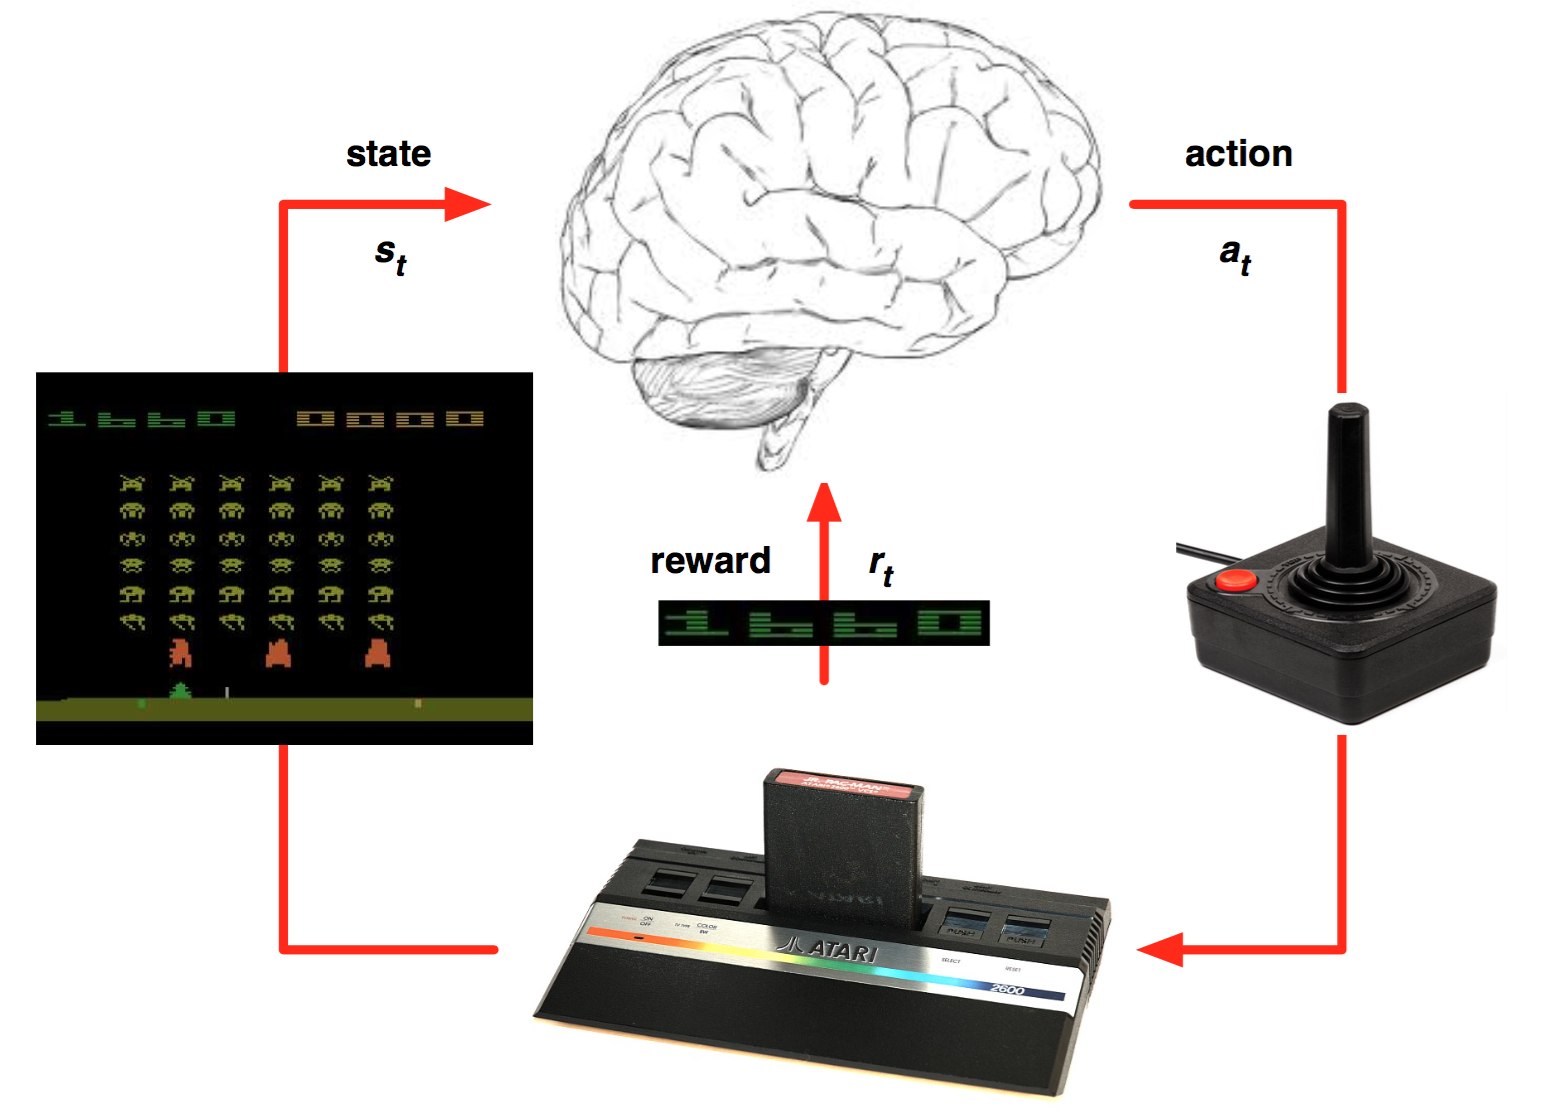
\includegraphics[width=\linewidth,keepaspectratio]{atari_rl.png}
	\caption{
		RL system to play Atari games (Source: \cite{mnih2013playing})
		}
	\label{img:atari_rl}
\end{figure}
% The rl system have 4 main compoentn s
In the figure \ref{img:atari_rl}, the brain represents the agent. Agent is our
computational system.
Agent in RL interacts with environment by performing actions. An action would be moving a joystick in the right.
By moving a joystick
we interact with environment, which in this case is the Atari video console.
After the environment receives an action, it gives back to the agent an observation
and reward signal. In our example, an observations is the current state of the game,
i.e. the image representing it and reward is the current score of the game.
\\
\paragraph{State}
Let's now abstract from our example and describe the flow of RL system more precisely.
At each time step $t$ the agent executes an action $A_t$, receives the observation $O_t$
and receives scalar reward $R_t$. The environment receives an action $A_t$,
emits observation $O_{t+1}$, emits scalar reward $R_{t+1}$. Then $t$ is incremented
after the environment's step. In RL instead of working with observations, one works
with the \emph{state} or \emph{agent state}. The agent state is the data the agent uses
to pick the next action. State is formally a function of the
history(data that agent received so far):
$H_t = O_1, R_1, A_1, O_2, R_2, A_2, ..., O_t, R_t, A_t$:

\begin{equation} \label{eq:rl_state}
	S_t = f(H_t)
\end{equation}

Because history $H_t$ can be very hard to maintain as it grows rapidly over the time,
it is very common to talk about \emph{markov state} in RL. Markov state is meant
to contain all useful information from the history as well as possess of \emph{markov property}:
\begin{equation} \label{eq:markov_property}
	P[S_{t+1} | S_t] = P[S_{t+1} | S_1, ..., S_t]
\end{equation}
where $S_t$ - is the state at time step $t$.
It means that the state is only dependent on the present state and not on
successors states. Hence, once the state is know, we can erase the history.

\paragraph{Reward} As mentioned before $R_t$ is scalar feedback signal, which
indicates how well agent is doing at time step $t$. The job of an agent to
maximise the sum of rewards received after $t$ steps. This sum is also known as
cumulative reward.

Additionally to this an agent may possess of following components:
% Beside the agent and environment, we can identify 4 main components used
% in RL systems:
a \emph{policy},
% a \emph{reward function},
a \emph{value function}, and,
optionally, a \emph{model of the environment}.

\paragraph{A Policy} is agent's behaviour function. It maps agent's state
to actions to be taken by agent, when agent are in those states. Normally, the policy is
something that we want to find. Once the best policy is known, we solved RL problem.
Policy can be deterministic: $a = \pi (s)$
as well as stochastic: $\pi(a|s) = P[A_t = a|S_t = s]$

% \paragraph{Reward function}

\paragraph{Value function} describes how good is it to be in a particular state.
% It maps a state to \emph{return} when following policy $\pi$. Return is cumulative
% reward from time step $t$ on if we follow the policy $\pi$.
The value of a state is the total amount of reward an agent can expect to
to receive when following policy $\pi$, starting from that state:

\begin{equation} \label{eq:markov_propert}
	v_{\pi}(s) = \mathbb{E}_{\pi} [R_{t+1} + \gamma R_{t+2} + \gamma^2 R_{t+3} + ... | St = s]
\end{equation}
where $\mathbb{E}_{\pi}$ is the expectation of the cumulative reward from time step $t$
following policy $\pi$ given the state $s$, $\gamma$ - is a discount factor which will be explained in \autoref{subs:reward_process}\\
While reward determines how well is current action at given time step, value of a state
give us more information about long term desirability of a state taking into account
the values of all possible states an agent can end up in after leaving this state.
It's crucial to understand the difference between reward and value: reward is immediate,
while the value giving us insights about the cumulative reward the agent can possibly get
from this state on.

\paragraph{Model of the environment} represents what the environment will do next. Given
the current state $s$ and action $a$, model defines the probability of an agent to end up in
a state $s^\prime$:
\begin{align} \label{eq:markov_propert}
P^a_{ss^{\prime}} = P[S_{t+1} = s_0 | S_t = s, A_t = a] \\
R^a_s = \mathbb{E}[R_{t+1} | S_t = s, A_t = a]
\end{align}
where $P$ is state transition probability matrix and $R$ is a reward function.

\subsection{Partially Observable Environments}
One distinguishes between two type of environments in RL problems.
\emph{Fully observable environments} where an agent is capable of directly observing the state of environment,
and \emph{partially observable environment}. In this work we will concentrate
on partially observable environments.

\paragraph{Partially observable environments}
In partially observable environments the agent's state is not equal to environment state,
instead the agent is constructing his own representation of environment state from
the the external input(observations) that the environment provide.
Partially observable environments is a special instance of what is known in RL community
as partially observable Markov decision process (POMDP). In our work we are constructing
the agent's state by injection the input into RNN:
\begin{equation} \label{eq:rnn_state}
	S_t^a = \sigma(S_{t-1}^a) \cdot W_s + O_t \cdot W_o)
\end{equation}
where $S_t^a$ and $S_{t-1}^a$ are agent state at time step $t$ and $t-1$
respectively, $O_t$ - is external input (in our work that is glimpse),
and $W_s$, $W_o$ - appropriate weights.
We will investigate in POMDP more in \autoref{subs:POMDP}.
% \paragraph{Partially Observable Environments}

% TODO: tomorrow
% explain the main ideas only behind  Markov decision process
% explain a bit about temporal difference algorithm
% explain reinforce

\subsection{Markov Reward Process} \label{subs:reward_process}

\subsection{POMDP} \label{subs:POMDP}




% write about main components
% * state
% * value
% * return and reward
% *
% about markov decision process
% about types of environments
%

% MOMDP
% Reinforce rule
% reducing variance by using advantage function
